%%%%%%%%%%%%%%%%%%% Figure 2 Bathymetry and currents in the Drøbak area %%%%%%%%%%%%%%%
\begin{figure}[t]
 \begin{center}
  \begin{pspicture}(0,0)(15,10.5)
% Include graphs
   \rput[bl]( 0,0){\includegraphics[height=11cm]{oslofjord_kart_ferder}}
   \rput[br](15,0){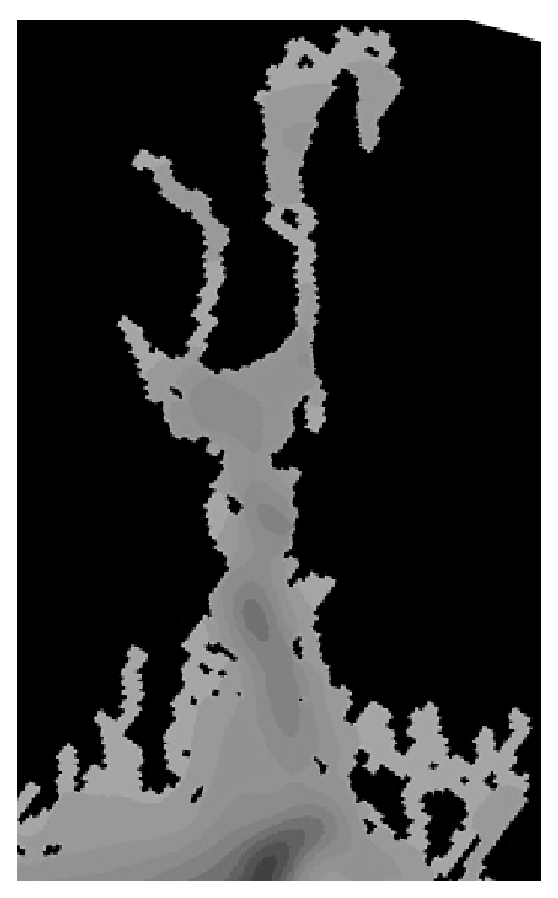
\includegraphics[height=11cm]{NorKyst800_topo_oslofjord}}
  \end{pspicture}
  \caption{\small The irregular coastline geometry and topography in the Oslofjord as portrayed in maps (left-hand panel) and the NorKyst800 model (right-hand panel). The red star sign marks the location of the F{\ae}rder lighthouse. Note the difference in size and depth of the major Hvalerdjupet basin near the southern boundary and the general smoothness of the NorKyst800 topography compared to the real topography.}
  \label{fig:hvaler2}
 \end{center}
\end{figure}

